\begin{frame}\frametitle{Parton distribution functions}
\centering\small

  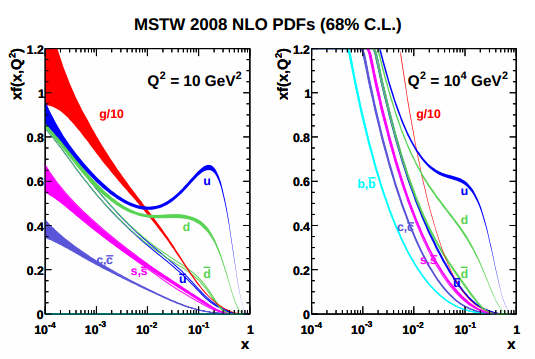
\includegraphics[width=0.6\textwidth]{../montecarlo/figures/pdfs2.png}

\myskip
standard PDFs $f_{a,b}(x_{a,b},\mu_{F})$ 
for partons $a,b = \{g,u,\bar{u},d,...\}$ 
 carrying fractions $x_a,x_b$ of the proton longitudinal momenta
$p_1, p_2$
\end{frame}



\begin{frame}\frametitle{Factorization theorem}
\centering\myskip

In any {\cccolor hard and inclusive} process ${\rm pp}\to{\rm X}$\\
can separate the {\cccolor soft} and {\cccolor hard} components:
$$
  \sigma_{{\rm pp}\to{\rm X}}
  = \sum_{a,b}
  \int_{0}^{1}{\rm d}x_a{\rm d}x_b
  ~ f_a(x_a,\mu_{F}) f_b(x_b,\mu_{F})
  \hat{\sigma}_{{\rm ab}\to{\rm X}}(x_ap_1, x_bp_2,\mu_R^2,\mu_{F}^2)
$$

short distance partonic cross section computable in fixed-order pQCD:
$$\hat{\sigma}_{{\rm ab}}=\sum_{i=0}^{n} \alphas^i \hat{\sigma}_i(x_ap_1, x_bp_2,\mu_R^2,\mu_{F}^2)=\hat{\sigma}_0+\alphas \hat{\sigma}_1+\dots$$

\begin{itemize}
\item $\mu_{F}$ = {\it factorization scale} 
\item arbitrary choice of the scale at which soft- and hard-interaction separate, in general $\mu_{R}$ (\alphas\ renormalization scale)
\end{itemize}

\end{frame}



\begin{frame}\frametitle{Multi-purpose Monte Carlo generators}
\centering\myskip

\begin{itemize}
\item \texttt{PYTHIA}: ME computed at LO for $2 \to n$ ($n\leq 3$) processes; PS with emissions
ordered in $p_T$ instead of angle; Lund string model used for hadronization
and UE simulation
\item \texttt{HERWIG}: ME computed at LO for $2 \to 2$ processes; PS with emissions ordered in angle;
cluster model used for hadronization and for the UE description; typically interfaced 
with the external package \texttt{JIMMY} for UE (MPIs in  $2 \to 2$ processes with the ME computed at LO)
\texttt{HERWIG} for the modeling of PS, hadronization and UE
\item \texttt{SHERPA}: modular design allowing NLO corrections; 
interfaced with \texttt{PYTHIA} for PS; ME/PS matching
performed with the CKKW scheme; hadronization done 
within \texttt{PYTHIA}
\end{itemize}

\end{frame}



\begin{frame}\frametitle{Specialized Monte Carlo generators}
\centering\myskip

\begin{itemize}
\item \texttt{ACERMC}: ME at LO; typically interfaced either with \texttt{PYTHIA} or 
\item \texttt{ALPGEN}: ME computation of $2 \to n$ ($n\leq 9$) events at LO; interfaced
with \texttt{PYTHIA} or \texttt{HERWIG} for PS and hadronization; ME/PS matching
in the MLM scheme; UE simulated through \texttt{PYTHIA};
%The various parton multiplicity samples are then normalized to their LO cross section and combined into an inclusive sample, which is finally typically normalized to an inclusive cross section calculated at higher order in pQCD. 
\item \texttt{MADGRAPH}: ME computation of $2 \to n$ ($n\leq 6$) events at LO;
interfaced with \texttt{PYTHIA} for PS, hadronization and UE;
MLM matching scheme
\item \texttt{MC@NLO}: ME at NLO allowing negative weighted events; 
higher-multiplicity parton emission beyond the first one simulated through PS in \texttt{HERWIG};
hadronization and UE simulated through \texttt{HERWIG}
\item \texttt{POWHEG}: ME at NLO; interfaced either with \texttt{PYTHIA} or 
\texttt{HERWIG} for PS, hadronization and UE
\end{itemize}


\end{frame}



\begin{frame}\frametitle{QCD Matrix Method}
\centering\scriptsize

Non-prompt electrons from:
\begin{itemize}
\item heavy flavor quark decays
\item photons mis-identified as electrons ($\gamma\to e^+ e^-$ conversion or random track overlap)
\item jets with high electromagnetic deposits mis-identified as electrons ($\pi^0$ and $\eta$ decays into two close-by photons)
\end{itemize} 

Non-prompt muons from semileptonic $b$- and $c$-hadron decays

\begin{minipage}{.35\textwidth}\centering

\includegraphics[width=1.\textwidth]{../vlq_analysis/figures/mm_regions}
\begin{eqnarray*}
N^\mathrm{loose} & = & N^\mathrm{loose}_\mathrm{real} + N^{loose}_\mathrm{fake}, \\
N^\mathrm{tight} & = & \epsilon_\mathrm{real}N^\mathrm{loose}_\mathrm{real} + \epsilon_\mathrm{fake}N^\mathrm{loose}_\mathrm{fake}.
\end{eqnarray*}

\end{minipage}\begin{minipage}{.65\textwidth}\centering

efficiencies of selecting real and fake loose leptons as tight leptons measured in dedicated control regions:
\begin{eqnarray*}
\epsilon_\mathrm{real} & = & \dfrac{N^\mathrm{tight}_\mathrm{real}}{N^\mathrm{loose}_\mathrm{real}}, \\
\epsilon_\mathrm{fake} & = & \dfrac{N^\mathrm{tight}_\mathrm{fake}}{N^\mathrm{loose}_\mathrm{fake}}.
\end{eqnarray*}

QCD background estimated as:\\
$N^\mathrm{tight}_\mathrm{fake} = \frac{\epsilon_\mathrm{fake}}{\epsilon_\mathrm{real} - \epsilon_\mathrm{fake}}(N^\mathrm{loose} \epsilon_\mathrm{real} - N^\mathrm{tight})$

\end{minipage}


\end{frame}



\begin{frame}\frametitle{QCD Matrix Method}
\centering\scriptsize

$\epsilon_\mathrm{fake}$ dependency on leading jet \pt\ and min$\Delta R(\mu,j)$:
\begin{itemize}
\item high leading jet \pt\ $\to$ higher hadronic activity nearby the lepton
\item muons closer to jets
\item isolation requirement $\min\Delta R(\mu,j)>0.4$ will fail! $\to$ lower $\epsilon_\mathrm{fake}$
\end{itemize}
more jets in events will contribute to these effects $\to$ Njets enters in the parametrization too

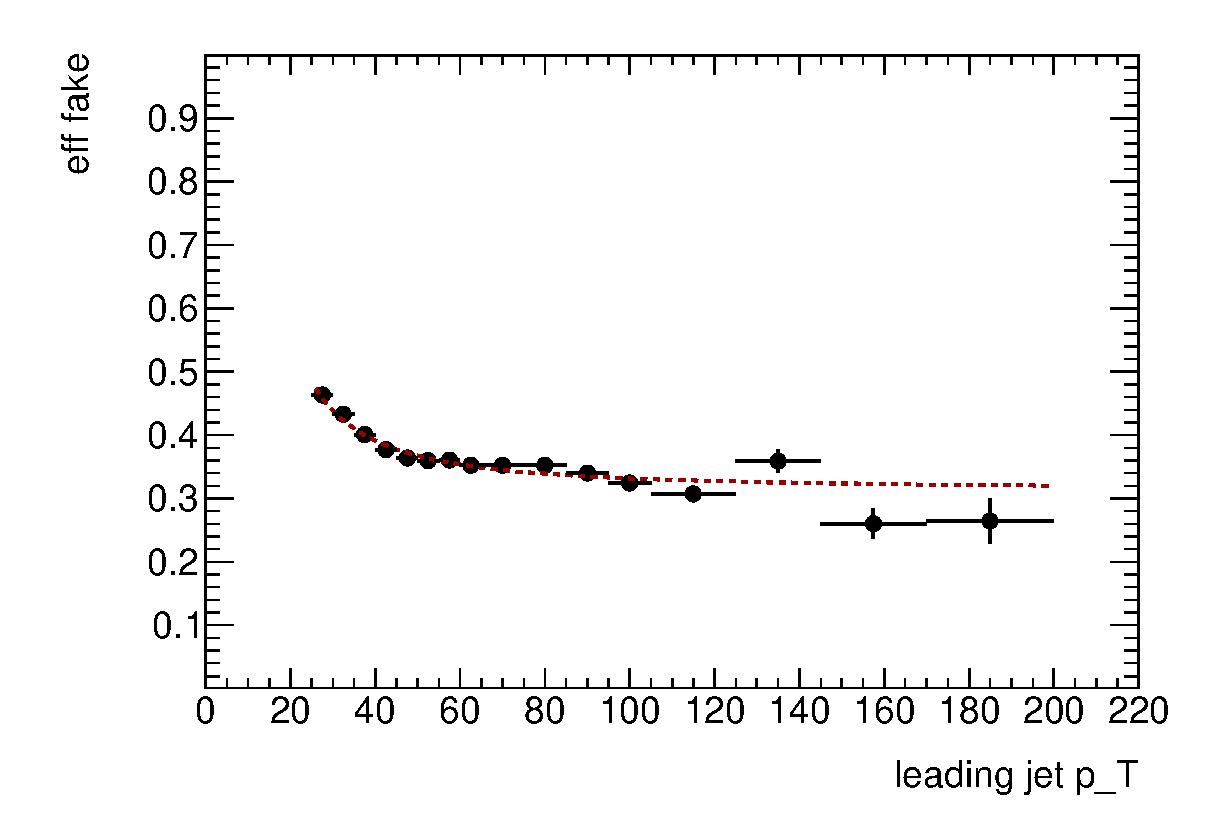
\includegraphics[width=.45\textwidth]{../appendices/figures/mujets_mmB/fit_h_lep_LJpT_rb_muon_fake_untagged}
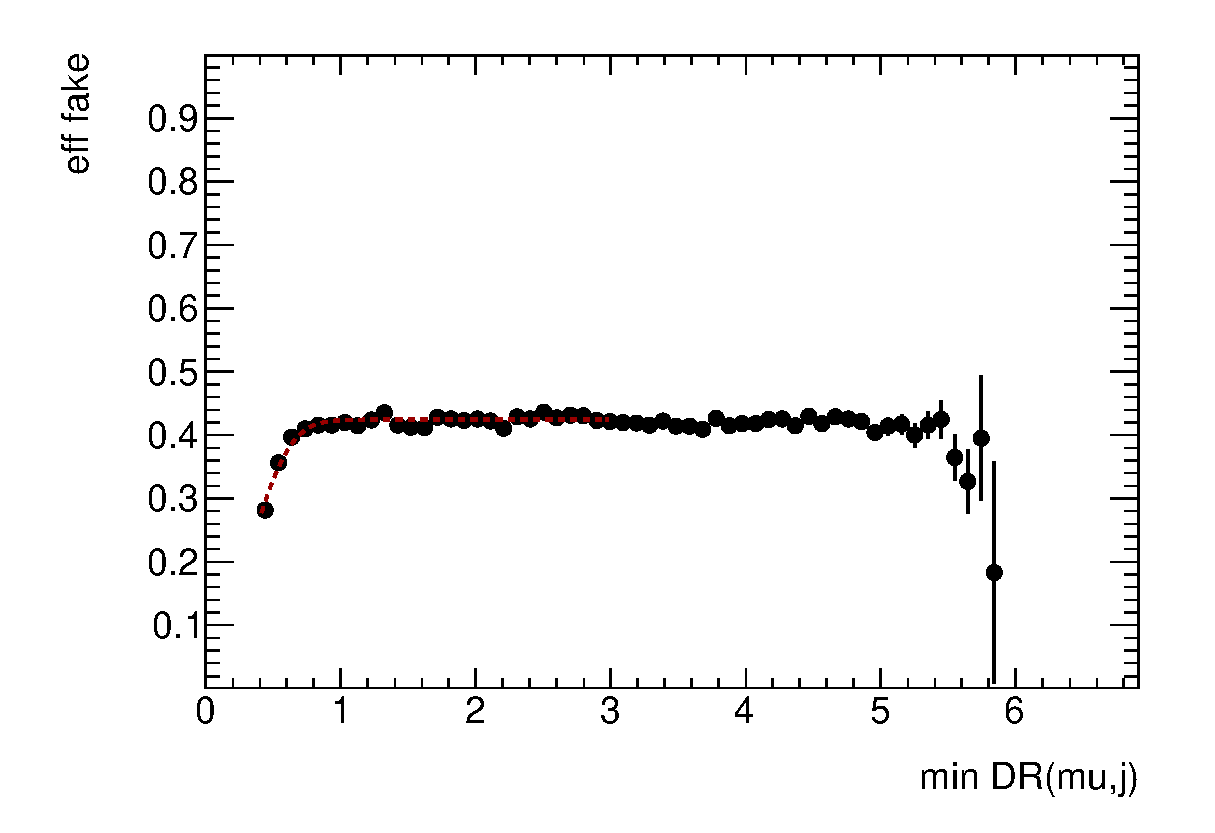
\includegraphics[width=.45\textwidth]{../appendices/figures/mujets_mmB/fit_h_lep_minDR_muon_fake_untagged}


\end{frame}



\begin{frame}\frametitle{Tag Rate Function method}
\centering\scriptsize

\begin{minipage}{.45\textwidth}\centering

Probability of a given event to contain the desired number of \btag ged jets
$$\Downarrow$$
Calculate event weight using the
per-jet  \btag ging efficiency

$$\varepsilon \left(\pt,|\eta|,f\right)$$

Event with $N$ jets: probability of 
containing exactly one $b$-tagged jet
$$P_{=1} = \sum\limits_{i=1}^N \left( \varepsilon_{i} \prod\limits_{j \neq i} \left( 1 - \varepsilon_{j} \right) \right)$$
\end{minipage}\begin{minipage}{.05\textwidth}\centering
$\,$
\end{minipage}\begin{minipage}{.5\textwidth}\centering

Probability of containing exactly $M$ $b$-tagged jets $\to$ iterate over all the possible subsets of $M$ and $N-M$ jets:
\begin{align*}
        P_{=M} &= \sum\limits_{i,\dots,m=1}^N 
        \left( 
        \prod\limits_{i=1}^{m=M} \varepsilon_{i}  
        \prod\limits_{j=m+1}^N \left( 1 - \varepsilon_{j} \right) 
        \right),
	%P_{=m} &= \sum\limits_{i,j,\dots,m=1}^N \left( \varepsilon_{i}\varepsilon_{j}\dots\varepsilon_{m}(1-\delta(i,j,\dots,m)) \prod\limits_{k \neq i\neq j \dots\neq m} \left( 1 - \varepsilon_{k} \right) \right), \\
\end{align*}

Probability for inclusive $b$-tagging selections:
\begin{align*}
	P_{=0} &= \prod\limits_{i=1}^N \left( 1 - \varepsilon_{j} \right), \\
	P_{\geq 1} &= 1 - P_{=0},\\
&\dots \notag\\
	P_{\geq m} &= 1 - \sum\limits_{i=0}^{m-1} P_{=i}.
\end{align*}
\end{minipage}

\end{frame}



\begin{frame}\frametitle{Tag Rate Function method}
\centering\scriptsize

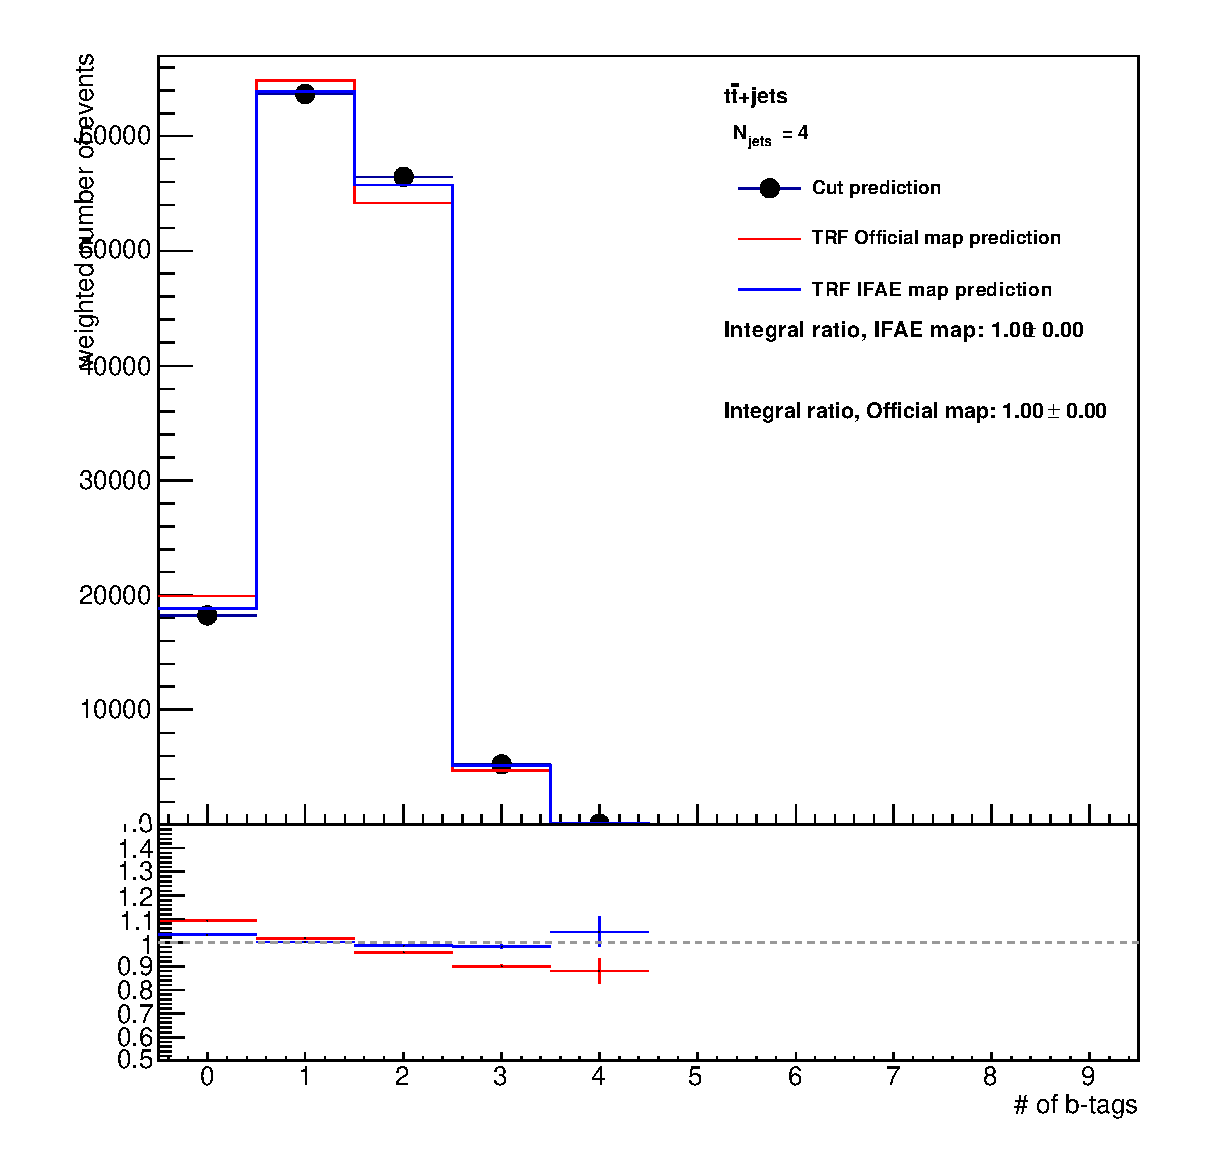
\includegraphics[width=.3\textwidth]{pics/ttbarAlpgen_HFOR_ntags_4jetex}
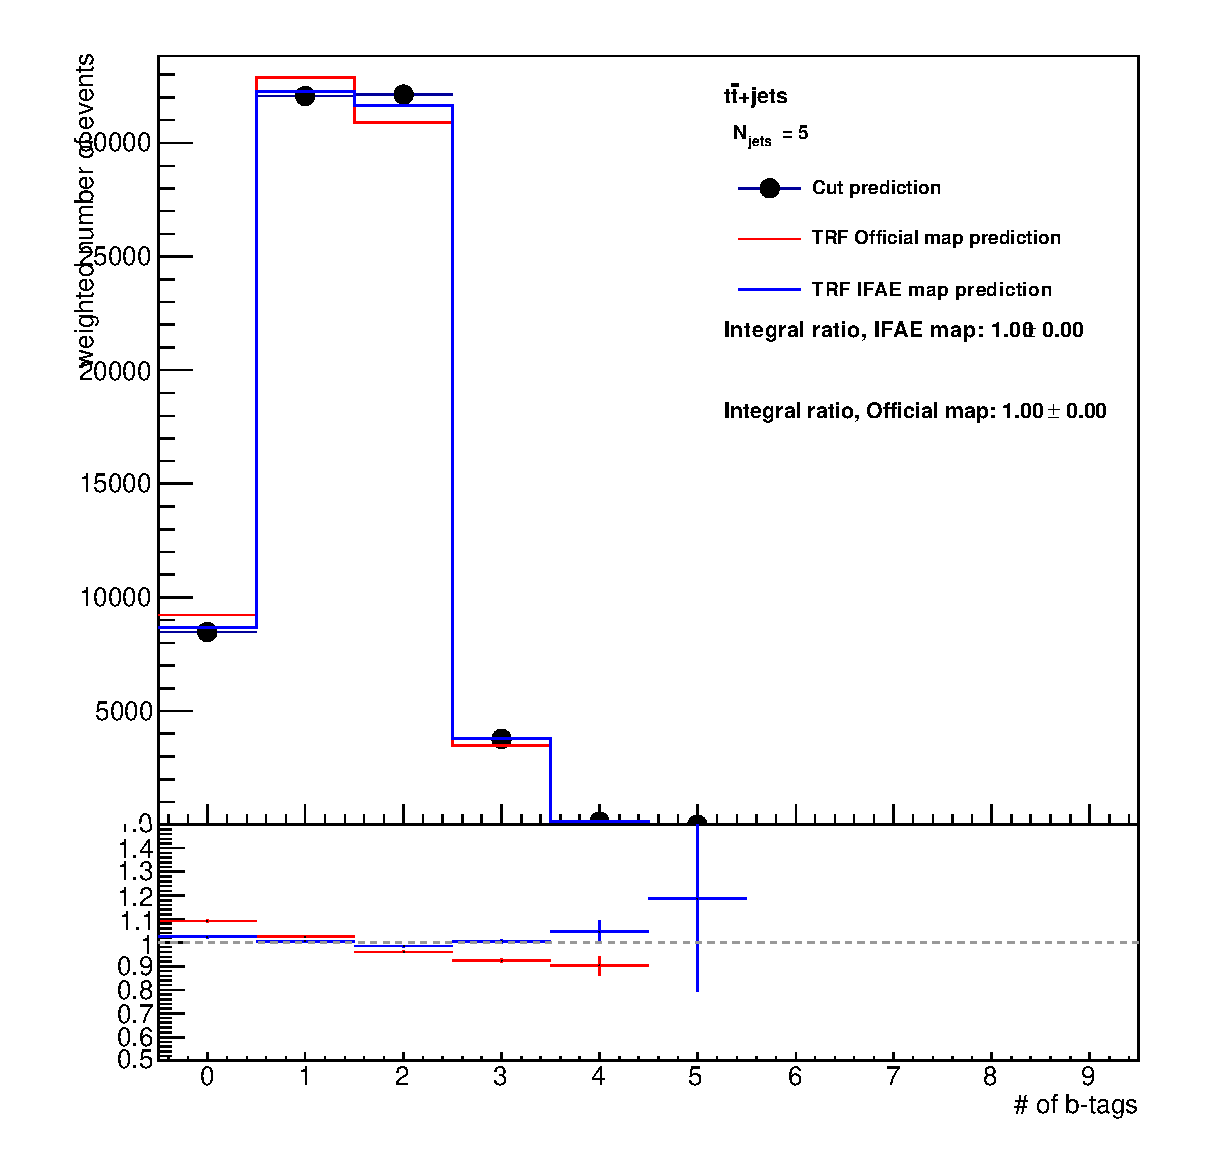
\includegraphics[width=.3\textwidth]{pics/ttbarAlpgen_HFOR_ntags_5jetex}
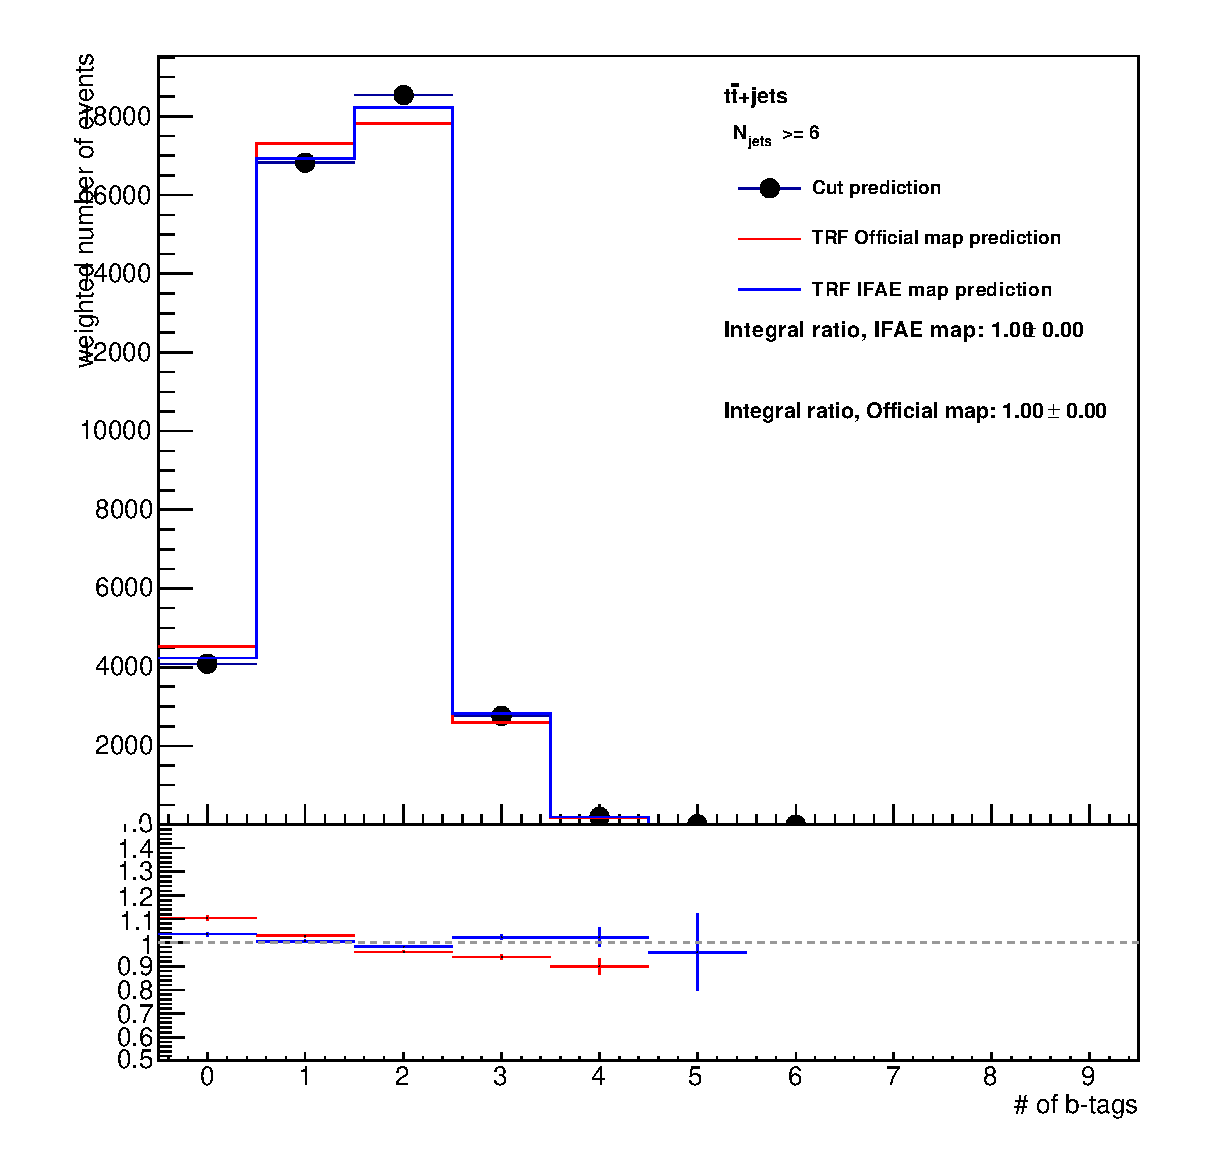
\includegraphics[width=.3\textwidth]{pics/ttbarAlpgen_HFOR_ntags_6jetin}

\tiny
\begin{tabular}{lcccc} \toprule
  & \multicolumn{2}{c}{TRF} & \multicolumn{2}{c}{Direct tagging}\\
  & Entries & Predicted yield & Entries & Predicted yield  \\
\midrule
\multicolumn{5}{c}{$W$+jets} \\
\midrule
Preselection            & 66381  & 37679.2 	$\pm$ 	324.0 	 & 8880  & 37317.3 	$\pm$ 	527.8 	\\
$\geq 1~W$              & 1321  & 723.2 	$\pm$ 	40.3 	 & 185  & 713.9 	$\pm$ 	66.7 	\\
$H_T>800~$GeV           & 520  & 314.0 	        $\pm$ 	27.4 	 & 84  & 308.0 	        $\pm$ 	41.7 	\\
$p_T(b_1) > 160~$GeV    & 262  & 146.9 	        $\pm$ 	17.8 	 & 44  & 155.3 	        $\pm$ 	30.5 	\\
$p_T(b_2) >80~$GeV      & 63  & 46.9 	        $\pm$ 	11.5 	 & 11  & 39.9 	        $\pm$ 	13.8 	\\
$\Delta R(l,\nu)<1.2$   & 28  & 16.3 	        $\pm$ 	6.0 	 & 5  & 14.7 	        $\pm$ 	7.2 	\\
min$\Delta R(l,b)>1.4$  & 15  & 6.3 	        $\pm$ 	2.8 	 & 2  & 5.2 	        $\pm$ 	4.0 	\\
min$\Delta R(W,b)>1.4$  & 9  & 5.5 	        $\pm$ 	2.8 	 & 1  & 3.7 	        $\pm$ 	3.7 	\\\bottomrule
\end{tabular}


\end{frame}



\begin{frame}\frametitle{$W$jets data-driven normalization}
\centering\scriptsize

Different 
cross sections for processes like
$\sigma(u\bar{d}\to W^+)$ and $\sigma(d\bar{u}\to W^-)$:\\
charge asymmetry predicted theoretically!

\myskip

$N_W=N_{W^+}+N_{W^-}$ estimated measuring $(N_{W^+}-N_{W^-})_{\rm meas}$ \\
i.e. difference between positively- and negatively-charged leptons

Compare MC prediction in the signal region (at least 4 jets):\\
$N_W = \left(\frac{N_{W^+}+N_{W^-}}{N_{W^+}-N_{W^-}}\right )_{\rm MC}(N_{W^+}-N_{W^-})_{\rm meas}$

\myskip 

Additional scale factors to account for flavor composition for $i=2$:
$$N^{W,{\rm tag}}_{i}  = 
N^{W,{\rm pretag}}_{i}
\sum_{x=b\bar{b}, c\bar{c}, c, light} F_{x,i}P_{x,i}$$

where $F_x$ are the flavor fractions $N^{\rm pretag}_x/N^{\rm pretag}$ 
(which add up to unity for each jet bin) and 
$P_x$ are the \btag ging probabilities for each flavor 
type $x = b\bar{b}, c\bar{c}, c, light$

\begin{itemize}
\item three unknown parameters need
to be fitted from data ($F_{c\bar{c},2}, F_{c,2}, F_{light,2}$).
\item $K_{x,i} = F^{\rm data}_{x,i}/F^{\rm MC}_{x,i}$
\end{itemize}
$F^{\rm MC}_{x,i}$ are the flavor fractions from simulation

\end{frame}



